\documentclass[a4paper,12pt]{article} 
\usepackage[T2A]{fontenc}			
\usepackage[utf8]{inputenc}			
\usepackage[english,russian]{babel}	
\usepackage{amsmath,amsfonts,amssymb,amsthm,mathrsfs,mathtools} 
\usepackage{cancel}
\usepackage{multirow}
\usepackage[colorlinks, linkcolor = blue]{hyperref}
\usepackage{upgreek}\usepackage[left=2cm,right=2cm,top=2cm,bottom=3cm,bindingoffset=0cm]{geometry}
\usepackage{graphicx,wrapfig,subfig}
\usepackage{tikz}
\usepackage{pgfplots}
\usepackage{xcolor}
\author{Трунов Владимир\\
Группа Б01-103}
\title{3.5.1. Изучение плазмы газового разряда в неоне.}
\date{}
\begin{document}

\begin{titlepage}
	\centering
	\vspace{5cm}
	{\scshape\LARGE Московский физико-технический институт \par}
	\vspace{4cm}
	{\scshape\Large Лабораторная работа 3.5.1 \par}
	\vspace{1cm}
	{\huge\bfseries Изучение плазмы газового разряда в неоне. \par}
	\vspace{7cm}
	\vfill
\begin{flushright}
	{\large Б01-103}\par
	\vspace{0.3cm}
	{\LARGE Трунов Владимир}
\end{flushright}
	

	\vfill

% Bottom of the page
	Долгопрудный, 2022 г.
\end{titlepage}

\textbf{Цель работы}: изучение вольт-амперной характеристики тлеющего разряда, изучение свойств плазмы методом зондовых характеристик.


\textbf{В работе используются}: стеклянная газоразрядная трубка, наполненная изотопом неона, высоковольтный источник питания (ВИП), источник питания постоянного тока, делитель напряжения, резистор, потенциометр, амперметры, вольтметры, переключатели.
\section*{Теория}
\subsection*{Плазма}
В ионизированном газе поле ионов <<экранируется>> электронами. Для поля $\mathbf{E}$ и плотности $\rho$ электрического заряда
$$
\text{div}~\mathbf{E} = 4 \pi \rho,
$$
а с учётом сферической симметрии и $\mathbf{E} = -\text{grad}~\varphi$:
\begin{equation}
\dfrac{d^2 \varphi}{dr^2}+\dfrac{2}{r}\dfrac{d\varphi}{dr}=-4\pi \rho.
\end{equation}
Плотности заряда электронов и ионов (которые мы считаем бесконечно тяжёлыми и поэтому неподвижными)
\begin{equation}
\begin{array}{c}
\rho_e = -ne \cdot \exp\left(\dfrac{e\varphi}{kT_e}\right),\\
\rho_i = ne.
\end{array}
\end{equation}
Тогда из $(1)$ в предположении $\dfrac{e\varphi}{kT_e} \ll 1$ получим
\begin{equation}
\varphi = \dfrac{Ze}{r}e^{-r/r_D},
\end{equation}
где $r_D = \sqrt{\dfrac{kT_e}{4\pi n e^2}}$ -- \textit{радиус Дебая}. Среднее число ионов в сфере такого радиуса 
\begin{wrapfigure}{r}{4cm}
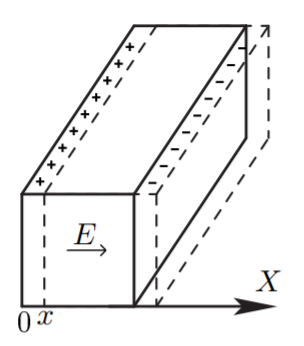
\includegraphics[scale=0.5]{2.png}
\end{wrapfigure}  
\begin{equation}
N_D = n\dfrac{4}{3}\pi r_D^2.
\end{equation}
Теперь выделим параллелепипед с плотностью $n$ электронов, сместим их на $x$. Возникнут поверхностные заряды $\sigma = nex$, поле от которых будет придавать электронам ускорение:
$$
\dfrac{d^2x}{dt^2}=-\dfrac{eE}{m}=-\dfrac{4\pi n e^2}{m}x.
$$ 
Отсюда получаем \textit{плазменную (ленгмюровскую) частоту} колебаний электронов:
\begin{equation}
\omega_p = \sqrt{\dfrac{4\pi ne^2}{m}}.
\end{equation}
\subsection*{Двойной зонд}
Двойной зонд -- система из двух одинаковых зондов, расположенных на небольшом расстоянии друг от друга, между которыми создаётся разность потенциалов, меньшая $U_f$. Рассчитаем ток между ними вблизи $I=0$. При небольших разностях потенциалов ионные токи на оба зонда близки к току насыщения и компенсируют друг друга, а значит величина результирующего тока полностью связана с разностью электронных токов. Пусть потенциалы на зондах
$$
U_1 = -U_f + \Delta U_1,
$$
$$
U_2 = -U_f + \Delta U_2.
$$
Между зондами $U = U_2 - U_1 = \Delta U_2 - \Delta U_1$.
Через первый электрод
\begin{equation}
I_1 = I_{i\text{н}} + I_{e1} = I_{i\text{н}} - \dfrac{1}{4}neS\langle v_e\rangle \exp\left(-\dfrac{eU_f}{kT_e}\right)\exp\left(\dfrac{e\Delta U_1}{kT_e}\right)=I_{i\text{н}}\left(1 - \exp\left( \dfrac{e\Delta U_1}{kT_e} \right)\right).
\end{equation}
Аналогично через второй получим
\begin{equation}
I_2 = I_{i\text{н}}\left(1 - \exp\left( \dfrac{e\Delta U_2}{kT_e} \right)\right)
\end{equation}
  
Из $(7)$ и $(8)$ с учётом последовательного соединение зондов ($I_1 = -I_2 = I)$:
$$
\Delta U_1= \dfrac{kT_e}{e}\text{ln}\left(1 - \dfrac{I}{I_{i\text{н}}}\right)
$$
$$
\Delta U_2= \dfrac{kT_e}{e}\text{ln}\left(1 + \dfrac{I}{I_{i\text{н}}}\right)
$$

Тогда итоговые формулы для разности потенциалов и тока

\begin{equation}
U = \dfrac{kT_e}{e}\text{ln}\dfrac{1 - I/I_{i\text{н}}}{1 + I/I_{i\text{н}}}, 
I = I_{i\text{н}} \text{th}\dfrac{eU}{2kT_e}.
\end{equation}
Реальная зависимость выглядит несколько иначе и описывается формулой 
\begin{wrapfigure}{l}{7cm}
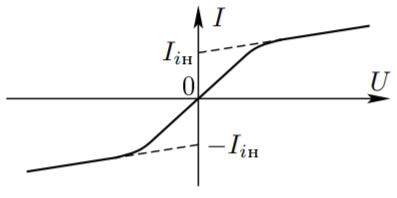
\includegraphics[scale=0.8]{4.png}
\vspace{+30pt}
\end{wrapfigure}
\begin{equation}
I = I_{i\text{н}} \text{th}\dfrac{eU}{2kT_e} + AU.
\end{equation}
Из этой формулы можно найти формулу для $T_e$: для $U=0$ мы найдём $I_{i\text{н}}$, продифференцируем в точке $U=0$ и с учётом $\text{th}~\alpha \approx \alpha$ при малых $\alpha$ и $A\rightarrow 0$ получим:
\begin{equation}
kT_e = \dfrac{1}{2}\dfrac{eI_{i\text{н}}}{\dfrac{dI}{dU}|_{U=0}}.
\end{equation}
\section*{Описание установки}
\begin{center}
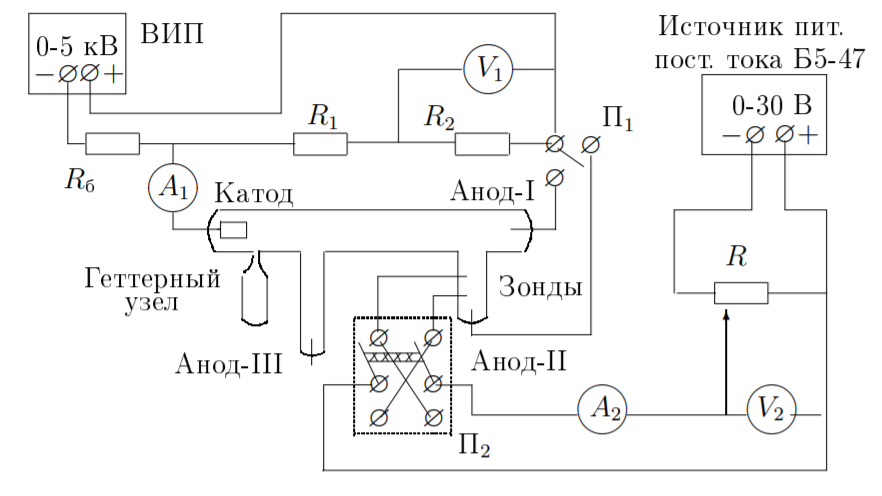
\includegraphics[scale=0.6]{1.png}
\end{center}
Стеклянная газоразрядная трубка имеет холодный (ненакаливаемый) полый катод, три анода и \textit{геттерный} узел -- стеклянный баллон, на внутреннюю повехность которого напылена газопоглощающая плёнка (\textit{геттер}). Трубка наполнена изотопом неона $^22$Ne при давлении 2 мм рт. ст. Катод и один из анодом (I и II) с помощью переключателя $\Pi_1$ подключается через балластный резистор $R_\text{б}$ ($\approx 450$ кОм) к регулируемому ВИП с выкодным напряжением до 5 кВ.\\
При подключении к ВИП анода-I между ним и катодом возникает газовый разряд. Ток разряда измеряется миллиамперметром $A_1$, а падение напряжения на разрядной трубке -- цифровым вольтметром $V_1$, подключённым к трубке черезе высокоомный (25 МОм) делитель напряжения с коэффициентом $(R_1+R_2)/R_2 = 10$.\\
При подключении к ВИП анода-II разряд возникает в пространстве между катодом и анодом-II, где находятся двойной зонд, используемый для диагностики плазмы положительного столба. Зонды изготовлены из молибденовой проволоки диаметром $d = 0.2$ мм и имеют длину $l = 5.2$ мм. Они подключены к источнику питания GPS через потенциометр $R$. Переключатель $\Pi_2$ позволяет изменять полярность напряжения на зондах. Величина напряжения на зондах изменяеься с помощью дискретного переключателя <<$V$>> выходного напряжения источника питания и потенциометра $R$, а измеряется цифровым вольтметром $V_2$. Для измерения зондового тока используется мультиметр $A_2$.

\end{document}